\section{IoT Gateway}
\label{sec:iotGateway}

Quando falamos de IoT (Internet das Coisas), já pensamos em que algo estará conectado à Internet. Essa "coisa"  não necessariamente se conecta de forma direta, sendo, na grande maioria dos casos, por meio um gateway ou roteador. IoT Gateway é uma aplicação (ou dispositivo com aplicação embarcado) responsável por receber requisições de diversos sensores e em algumas situações executar ações.

O gateway é similar a um roteador, porém, ele pode unir redes de diferentes protocolos, através de um processamento local para a tradução e conversão de protocolos. Gateways são muito utilizados em ambiente industrial e corporativo, porém, com o avanço do IoT, está ficando mais comum encontrar esse tipo de equipamento para uso residencial.

Atualmente fala-se em 2 tipos de IoT Gateways, os Traditional Gateways que não são inteligentes e apenas armazenam a informações para futura transmissão, e os Smart Gateways que além disso, podem fazer ações, tais como:
\begin{itemize}
	\item Persistir as informações
	\item Efetuar transformação dos dados recebidos
	\item Guardar os dados temporariamente para posteriormente transmiti-los para a web
	\item Executar regras de segurança sobre os dispositivos
	\item Executar ações com base nos dados recebidos e regras configuradas
\end{itemize}

A Figura \ref{fig:arquiteturaIotGateway} ilustra uma arquitetura convencional de um IoT Gateway e suas relações com os sensores e com a Cloud.

\begin{figure}[H]
	\centering
	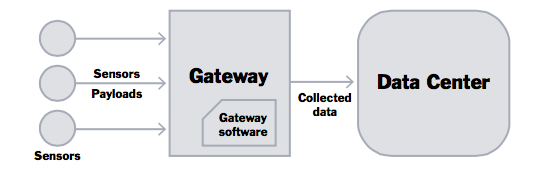
\includegraphics[width=0.9\textwidth]{./img/rumFxS7.png}
	\caption{Arquitetura de um IoT Gateway}
	\label{fig:arquiteturaIotGateway}
\end{figure}


Sensores residem no que a indústria nomeia como sendo campo, ou seja, onde os sensores realmente devem atuar. São exemplos de campos galpões, plantas industriais, florestas, plantações etc.

Já a Cloud tem o mesmo significado que estamos habituados: um servidor na nuvem onde dados são mantidos e processamentos são realizados.

O IoT Gateway faz esse meio de campo, uma vez que sensores não costumam ter boas condições de acesso à Internet, tanto do ponto de vista da disponibilidade quanto da velocidade.

A grande vantagem em fazer o seu próprio gateway, é o nível de customização que ele pode ter, já que temos total acesso ao sistema operacional, sem restrições impostas pelo fabricante – o que ocorre na maioria dos casos. Essa customização vai permitir usar o gateway em modo \textit{fog computing} (computação em nevoeiro), para o processamento de informações o mais perto do dispositivo da borda, ou edge device, fazendo com que, mesmo na falta de Internet, o dispositivo consiga se manter operacional, ainda que com algumas restrições.

Fazer o seu próprio gateway de IoT pode parecer loucura, mas com a baixa nos preços dos SoC’s (System-on-a-Chip), alavancado principalmente pela Raspberry Pi \cite{RaspberryPi}, torna possível a criação de sistemas computacionais de bom desempenho, tamanho reduzido e baixo custo. Já é possível encontrar SoC’s custando menos de US\$ 10 e chips completos e funcionais por menos de US\$ 40.